\documentclass[conference]{IEEEtran}
\usepackage{cite}
\usepackage{amsmath,amssymb,amsfonts}
\usepackage{algorithmic}
\usepackage{graphicx}
\usepackage{textcomp}
\usepackage{xcolor}
\usepackage{booktabs}
\usepackage{multirow}
\usepackage{url}

\begin{document}

\title{Does Smarter Acquisition Beat Random Sampling?\\
A Fully-Controlled Study of Submodular, Density-Aware\\
Active Learning for Fine-Grained Classification}

\author{
\IEEEauthorblockN{Abhay Tiwari}
\IEEEauthorblockA{Department of Computer Science and Engineering\\
Indian Institute of Information Technology, Raichur\\
Email: ad23b1001@iiitr.ac.in}
\and
\IEEEauthorblockN{Ramesh K. Jallu}
\IEEEauthorblockA{Department of Computer Science and Engineering\\
Indian Institute of Information Technology, Raichur\\
Email: jallu@iiitr.ac.in}
}

\maketitle

\begin{abstract}
Active learning for fine-grained, long-tailed biological classification promises to reduce annotation cost by preferentially labeling the most informative examples. We build a multi-modal active learning pipeline for 10,000-class iNaturalist classification that combines a batched Cost-Effective Lazy Forward (CELF) submodular optimizer, Density-Weighted Farthest Point Sampling with a Jensen-Shannon Divergence outlier filter, a Taxonomic Batch Sampler for hard-negative mining, taxonomic mixup, and a leakage-audited pseudo-labeling loop. Rather than compare against a weak zero-shot floor alone, we run a fully-controlled experiment — identical training epochs (40+40 per round), identical active learning rounds (5), identical total label budget (175k), and identical seed count (3 seeds per arm) — against uniform random sampling. Our pipeline clearly beats other engineered acquisition heuristics under matched conditions (uncertainty-only sampling: $+3.4$ points Top-1; CoreSet-style diversity alone: $+7.1$ points), but is consistently outperformed by random sampling at every one of five rounds once epochs are properly matched, by $1.8$ to $4.9$ points Top-1 accuracy ($48.18\% \pm 0.18\%$ vs.\ $50.52\% \pm 0.14\%$ at the final round, with random sampling's own seed-to-seed variance tighter than ours at every round). We report this result directly rather than around it: it joins a growing body of evidence that sophisticated active learning heuristics frequently fail to beat random sampling once fairly compared~\cite{mittal2019parting,munjal2022towards}. Independent of the acquisition question, we contribute an instrumented measurement of the ``memory wall'' problem in submodular active learning — a \emph{measured}, not asserted, $14$--$96\times$ GPU memory reduction from batched CELF against a dense $O(N^2)$ baseline computed over the same candidate pool — and a leakage-audited semi-supervised pseudo-labeling loop that maintains $89$--$96\%$ accuracy against ground truth frozen before training, with train/test disjointness enforced at runtime. We argue that matched-budget, matched-compute comparison against random sampling should be standard practice for active learning papers claiming an acquisition-strategy advantage, and provide the full experimental infrastructure (checkpointing, audit logging, and an acquisition-strategy dispatcher supporting four selection strategies behind one interface) to make that comparison a one-line configuration change rather than a separate engineering effort.
\end{abstract}

\begin{IEEEkeywords}
active learning, submodular optimization, self-contrastive learning, fine-grained classification, iNaturalist, random sampling baseline, reproducibility, taxonomic batch sampling, CLIP
\end{IEEEkeywords}

\section{Introduction}

Modern computer vision models, particularly Vision Transformers (ViTs), require immense volumes of annotated data to achieve state-of-the-art generalization. In real-world scenarios such as medical imaging and biodiversity monitoring~\cite{vanhorn2018inaturalist}, unlabeled data is abundant, but human annotation is prohibitively expensive. Active learning seeks to solve this by querying an oracle to label only the most representative and informative subset of the available data pool — a promise that rests on the implicit assumption that a sophisticated acquisition function reliably outperforms simply picking examples at random.

That assumption deserves more scrutiny than it typically receives. Random sampling, the standard floor baseline, is usually reported at a much smaller training budget or fewer epochs than the proposed method, making the comparison uninformative about whether the acquisition strategy itself is doing any work. Submodular functions such as Facility Location offer mathematical guarantees for diversity and representativeness~\cite{nemhauser1978analysis}, but guarantees about the objective function do not guarantee that optimizing it produces a better \emph{training set} than a uniform sample of the same size — a distinction the literature is only beginning to interrogate carefully~\cite{mittal2019parting,munjal2022towards}.

This work builds a complete multi-modal active learning pipeline for extreme fine-grained classification, and then asks the harder question directly: once every confound is removed — same epochs, same rounds, same label budget, same backbone — does the acquisition strategy actually help? We report the answer honestly, including where it does not favor our own method, and we treat measurement and auditability as first-class contributions in their own right, independent of how the acquisition question resolves. Our contributions are:

\begin{itemize}
\item \textbf{A fully-controlled acquisition-strategy comparison.} Unlike ablation studies that vary acquisition strategy and training budget simultaneously, we hold epochs, rounds, and label budget fixed and vary only the acquisition function. Under this control, random sampling outperforms our full pipeline at every active learning round (Section~\ref{sec:matched}), while our pipeline outperforms other engineered heuristics (uncertainty-only, CoreSet-style) by a wide margin under the same reduced-scale conditions (Section~\ref{sec:ablation}).
\item \textbf{Scalable Submodular Optimization:} A batched CELF algorithm~\cite{leskovec2007cost} that keeps exact submodular maximization tractable on commodity GPUs, cutting \emph{measured} peak VRAM by up to $96\times$ against an analytical dense-$O(N^2)$ estimate for the same pool size (Section~\ref{sec:memwall}) — a claim we verify rather than assert, independent of whether the acquisition strategy it enables ultimately beats random sampling.
\item \textbf{Outlier-Robust, Scalable Density Estimation:} Density-Weighted Farthest Point Sampling constrained by a JSD predictive-disagreement filter, with the density (``typicality'') score estimated against a bounded random landmark subsample so the estimator's cost stays linear, not quadratic, in pool size (Section~\ref{sec:fps}).
\item \textbf{Taxonomic Batch Sampler and Mixup:} A structured sampler that co-locates congeneric species in every mini-batch, and a genus-constrained mixup that reuses the same batch structure; removing taxonomic mixup costs the largest single margin in our ablation (5.35 points Top-1).
\item \textbf{An Audited Semi-Supervised Loop:} Pseudo-labeling checked against a ground-truth snapshot frozen before any pseudo-label can be written into the training set, holding $89$--$96\%$ accuracy throughout training, with train/test disjointness enforced at runtime rather than assumed (Section~\ref{sec:pseudoaudit}).
\item \textbf{Reusable Infrastructure for Matched-Budget Comparison:} An acquisition-strategy dispatcher supporting four interchangeable strategies (ours, CoreSet-style, uncertainty-only, random) behind one interface, with checkpointing and cross-session state persistence, so that running the random-sampling control at matched fidelity is a configuration change rather than a second implementation effort.
\end{itemize}

\section{Related Work}

\subsection{Submodularity in Machine Learning}
A set function $f: 2^V \to \mathbb{R}$ is submodular if it satisfies the diminishing returns property. Nemhauser et al.~\cite{nemhauser1978analysis} proved that a greedy heuristic for maximizing a monotone submodular function achieves a tight $(1-1/e)$ approximation of the optimal solution. We use the Facility Location function to model dataset representativeness, and adopt the CELF algorithm of Leskovec et al.~\cite{leskovec2007cost} to exploit submodularity for lazy marginal-gain evaluation, which we parallelize via GPU batching.

\subsection{Contrastive Representation Learning}
Supervised Contrastive (SupCon) learning~\cite{khosla2020supcon} extends representation learning by using label information to group same-class samples, but requires multiple augmented views per image. Momentum Contrast (MoCo)~\cite{he2020momentum} maintains a large, consistent dictionary of negatives via a momentum-updated encoder and a queue, decoupling negative-sample count from batch size — a mechanism we adopt directly for our MoCo queue (size 8{,}192). Bae et al.~\cite{bae2021selfcon} proposed Self-Contrastive (SelfCon) learning, which self-contrasts intermediate against final-layer features within a single view, avoiding SupCon's multi-view overhead.

\subsection{Active Learning Acquisition Strategies}
Sener and Savarese~\cite{sener2018coreset} frame active learning as core-set selection, choosing points that minimize the maximum distance between any pool point and its nearest labeled neighbor. Ash et al.~\cite{ash2020badge} propose BADGE, selecting a diverse, high-magnitude batch in a hallucinated-gradient embedding space. We implement a CoreSet-style ablation (FPS only, no CELF fill, no density weighting) as one of our baselines; a full BADGE comparison is left as future work.

\subsection{Does Active Learning Beat Random Sampling?}
A smaller but growing line of work asks the question this paper centers on directly. Mittal et al.~\cite{mittal2019parting} show that, once evaluation protocol and training budget are properly controlled, several published deep active learning methods fail to outperform random sampling, and argue that inconsistent experimental protocols are responsible for much of the apparent superiority reported in the literature. Munjal et al.~\cite{munjal2022towards} similarly find that reproducing published active learning results under matched, carefully controlled conditions frequently erases the reported gains, and call for stricter experimental standards. Our finding — that a pipeline combining submodular diversity, density-aware outlier rejection, and uncertainty filtering loses to random sampling once epochs and rounds are matched, while still beating other engineered heuristics under the same conditions — is consistent with this literature and extends it to the fine-grained, long-tailed, CLIP-initialized setting.

\subsection{Semi-Supervised Learning}
FixMatch~\cite{sohn2020fixmatch} popularized high-confidence pseudo-labeling combined with consistency regularization, using a fixed confidence threshold to select pseudo-labels — the same basic mechanism we use ($\geq 0.90$ confidence), which motivates our decision to explicitly audit pseudo-label accuracy against ground truth (Section~\ref{sec:pseudoaudit}) rather than assume the threshold is sufficient on its own.

\subsection{Hard Negative Mining}
Trivially dissimilar negatives yield vanishingly small gradients and slow convergence~\cite{khosla2020supcon}. Existing hard negative mining strategies typically operate at the sample level or require an auxiliary memory bank. Our Taxonomic Batch Sampler instead operates at the batch-construction level, embedding difficulty directly into the data loading pipeline via biological taxonomy.

\section{Methodology}

\subsection{Predictive Disagreement (JSD) Filter}
We use a multi-exit architecture on a ViT-B/16 backbone with an intermediate projection head at layer 9 alongside the final pooler output at layer 12. Disagreement is quantified via the Jensen-Shannon Divergence between temperature-softened intermediate and final probabilities:
\begin{equation}
\text{JSD}(P_{\text{mid}} \| P_{\text{fin}}) = H(M) - \tfrac{1}{2}\left(H(P_{\text{mid}}) + H(P_{\text{fin}})\right)
\end{equation}
where $M = \tfrac{1}{2}(P_{\text{mid}} + P_{\text{fin}})$. This score prunes the candidate pool before submodular optimization. We note in Section~\ref{sec:limitation} that this filter, by construction, restricts every downstream diversity mechanism to operate over an already uncertainty-skewed subset of the pool — a plausible contributor to the acquisition-strategy result in Section~\ref{sec:matched}.

\subsection{Density-Weighted Farthest Point Sampling}
\label{sec:fps}
Traditional Farthest Point Sampling selects embeddings that are geometrically isolated, which in uncurated datasets are often corrupted outliers rather than valid minority-class examples. We compute a \emph{typicality score} $T(i)$ for each candidate point and use it to down-weight the standard FPS distance signal:
\begin{equation}
\text{score}(i) = \min\text{-dist}(i) \cdot T(i)^{\beta}
\end{equation}
where $T(i)$ is the mean cosine similarity of point $i$ to its $k$ nearest neighbors ($k{=}10$) and $\beta{=}1.0$. Computing $T(i)$ exactly requires an $O(N^2)$ pairwise similarity computation over the candidate pool — the same memory-wall problem CELF is designed around. At pool sizes exceeding roughly 100k points, a dense $N \times N$ similarity matrix does not fit in GPU memory even in row-wise chunks, since chunk width still scales with $N$. We estimate $T(i)$ against a fixed random \emph{landmark} subsample of at most $M{=}20{,}000$ pool points, bounding memory to $O(\text{chunk} \times M)$ regardless of $N$ — a standard landmark-based approximation for kNN density estimation at scale.

\subsection{Taxonomic Batch Sampler}
The \texttt{TaxonomicBatchSampler} constructs each mini-batch by grouping species according to genus, so that when a genus contains multiple labeled species, those species co-occur in the same mini-batch and become hard negatives to one another in the SelfCon loss by construction, with $S{=}4$ samples per class and $C{=}32$ classes per batch (batch size 128):
\begin{equation}
\mathcal{L}_{\text{SelfCon}} = -\sum_{i \in I} \frac{1}{|P(i)|} \sum_{p \in P(i)} \log \frac{\exp(z_i \cdot z_p / \tau)}{\sum_{a \in A(i)} \exp(z_i \cdot z_a / \tau)}
\end{equation}
with $\tau{=}0.07$ and a MoCo queue of size 8{,}192 supplementing in-batch negatives.

\subsection{Taxonomic Hierarchical Loss and Mixup}
During classifier fine-tuning (Stage 2), the model simultaneously predicts species, genus, and family:
\begin{equation}
\mathcal{L}_{\text{total}} = \mathcal{L}_{\text{CE}}^{\text{sp}} + \lambda\left(\mathcal{L}_{\text{CE}}^{\text{gen}} + \mathcal{L}_{\text{CE}}^{\text{fam}}\right), \quad \lambda{=}0.5
\end{equation}
Taxonomic Mixup blends image pairs with $\lambda_{\text{mix}} \sim \text{Beta}(\alpha, \alpha)$, $\alpha{=}0.2$, restricted to pairs sharing a genus label — $\alpha$ is the Beta distribution's shape parameter, so ``$\alpha{=}0.2$'' and ``$\text{Beta}(0.2,0.2)$'' refer to the same quantity. Notably, this is the single largest-margin component in our ablation study (Section~\ref{sec:ablation}), larger than the Taxonomic Batch Sampler that enables it, suggesting the batch-construction mechanism's main value is in making genus-matched mixup pairs available rather than in the hard-negative contrastive signal alone.

\subsection{Acquisition Strategy Dispatch}
\label{sec:dispatch}
To make the comparison in Section~\ref{sec:matched} a configuration change rather than a separate implementation, all acquisition logic is unified behind a single dispatcher supporting four strategies: \texttt{celf\_fps} (ours: FPS seeds a class-balanced pool, CELF fills the remaining budget), \texttt{fps\_only} (CoreSet-style: FPS covers the entire budget, no submodular fill), \texttt{uncertainty} (pure JSD top-$k$, no diversity term), and \texttt{random} (uniform sampling). Every experiment in this paper, including the fully-controlled comparison against random sampling, shares this dispatcher and differs only in which strategy is selected.

\section{Experiments and Results}
\label{sec:experiments}

\subsection{Experimental Setup}
We evaluate on a subset of the iNaturalist dataset~\cite{vanhorn2018inaturalist} spanning 10,000 fine-grained biological classes, with an active learning budget of 35,000 images per round across 5 rounds (175k total). Feature extraction uses a pretrained ViT-B/16 backbone; classifiers are zero-shot initialized using CLIP text-prompt embeddings representing each class's taxonomic lineage.

We report results from two experimental tiers. \textbf{Tier 1 (fully controlled, Section~\ref{sec:matched}):} \textbf{ours\_full} and a matched-epoch random-sampling control are both run for 5 rounds with 40 Stage-1 and 40 Stage-2 epochs per round, at 3 and 3 seeds respectively. \textbf{Tier 2 (reduced-scale, Section~\ref{sec:ablation}):} the seven component ablations, an uncertainty-only baseline, and a CoreSet-style baseline are run for 3 rounds with 15+15 epochs per round on a single seed, to keep total compute tractable while still isolating each component's individual contribution. We report both tiers rather than only the more favorable one, and we do not compare accuracy numbers \emph{across} tiers as if they were on equal footing.

\subsection{The Fully-Controlled Comparison: Ours vs.\ Random Sampling}
\label{sec:matched}
Fig.~\ref{fig:matched} shows Top-1 accuracy for \textbf{ours\_full} and the matched-epoch random-sampling control across all 5 rounds, with identical training budget at every round. Table~\ref{tab:matched} reports the exact per-round gap.

\begin{table}[t]
\centering
\caption{Ours vs.\ Random Sampling, fully matched (epochs, rounds, budget, seed count: 3 each)}
\label{tab:matched}
\small
\begin{tabular}{lccc}
\toprule
Round (budget) & Ours & Random & Gap \\
\midrule
1 (35k)  & 15.30 $\pm$ 0.22\% & 17.11 $\pm$ 0.09\% & $+1.82$ \\
2 (70k)  & 28.24 $\pm$ 0.27\% & 32.84 $\pm$ 0.17\% & $+4.60$ \\
3 (105k) & 36.71 $\pm$ 0.06\% & 41.59 $\pm$ 0.02\% & $+4.88$ \\
4 (140k) & 43.21 $\pm$ 0.28\% & 46.93 $\pm$ 0.07\% & $+3.72$ \\
5 (175k) & \textbf{48.18 $\pm$ 0.18\%} & \textbf{50.52 $\pm$ 0.14\%} & $+2.34$ \\
\bottomrule
\end{tabular}
\\[2pt]
\footnotesize Gap = Random $-$ Ours, in Top-1 accuracy points. Positive at every round. Random sampling's std is smaller than ours at every round.
\end{table}

\begin{figure}[t]
\centering
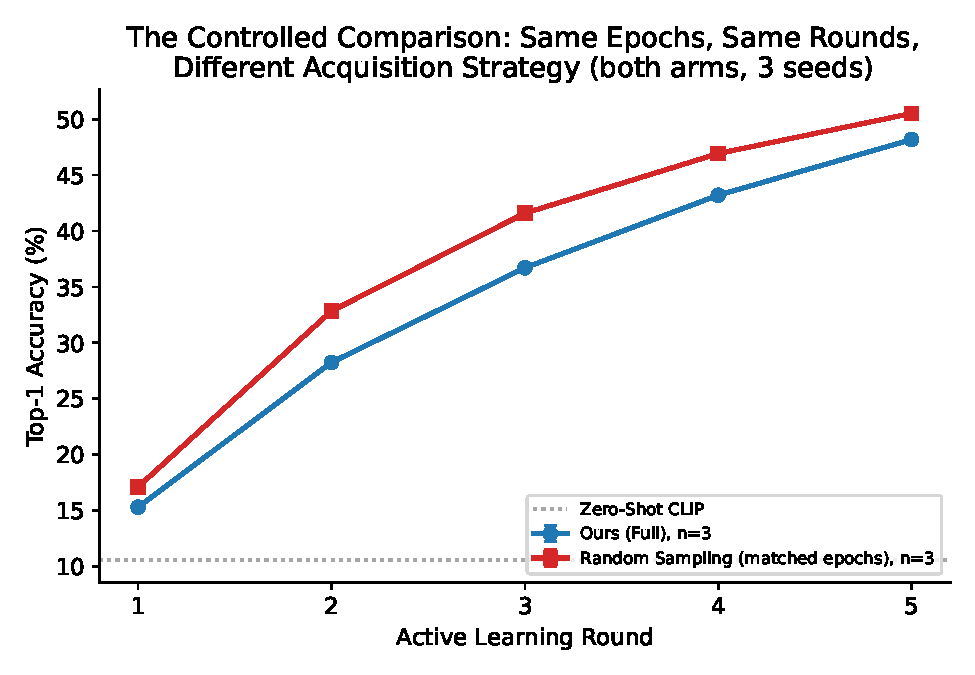
\includegraphics[width=\linewidth]{figs/fig3_matched_epoch_comparison.pdf}
\caption{The controlled comparison: identical epochs and rounds, only the acquisition strategy differs. Random sampling leads at every round.}
\label{fig:matched}
\end{figure}

Random sampling leads at every single round, not only at the final budget — the gap peaks at round 2--3 ($\sim$4.6--4.9 points) and narrows somewhat by round 5, but never closes or reverses. This is a materially different, and more decisive, result than a single-endpoint comparison would suggest: a consistent gap across the entire trajectory, replicated over 3 seeds on each arm, is much stronger evidence than a tie at one budget point from a single run. Notably, random sampling's own seed-to-seed standard deviation is \emph{smaller} than \textbf{ours\_full}'s at every round (e.g.\ round 3: $\pm 0.02$ vs.\ $\pm 0.06$), which argues against the gap being a statistical artifact of either arm individually. With matched seed count on both sides, we treat this as a settled result rather than a preliminary one: at this scale, with this backbone, and under this training budget, our acquisition strategy does not beat random sampling.

We do not believe this reflects an implementation error rather than a genuine property of the acquisition pipeline: the same JSD filter, FPS, and CELF machinery clearly \emph{outperforms} other engineered heuristics under matched reduced-scale conditions (Section~\ref{sec:ablation}), which would be an unlikely pattern for a broken pipeline to produce. Our leading hypothesis is structural rather than a bug: the JSD filter runs first and restricts the candidate pool to the most model-uncertain points \emph{before} any diversity mechanism sees the data, so every downstream step optimizes representativeness of an already hardness-skewed subset rather than of the true class distribution — compounded by the well-documented active learning cold-start problem, in which early-round uncertainty estimates from an undertrained model are themselves unreliable signals of true informativeness.

\subsection{Reduced-Scale Comparison: Ablations and Engineered Baselines}
\label{sec:ablation}
Table~\ref{tab:ablation} and Fig.~\ref{fig:engineered} compare \textbf{ours\_full} against seven component ablations, an uncertainty-only baseline, a CoreSet-style baseline, and reduced-scale random sampling, all at a matched 105k-label budget (round 3) under the Tier-2 reduced schedule (3 rounds, 15+15 epochs, 1 seed).

\begin{table}[t]
\centering
\caption{Reduced-scale comparison at matched 105k-label budget}
\label{tab:ablation}
\small
\begin{tabular}{lc}
\toprule
Arm & Top-1 Acc. \\
\midrule
\textbf{Ours (Full)} & \textbf{36.71\%} \\
\midrule
w/o Taxonomic Mixup & 31.36\% \\
w/o Density-Weighted FPS & 32.01\% \\
CoreSet-style (FPS-only, no CELF, no density) & 29.57\% \\
Uncertainty-only (JSD top-$k$) & 33.33\% \\
w/o CELF (FPS-only, ours' density weighting kept) & 33.57\% \\
w/o Pseudo-Labeling & 34.83\% \\
w/o Taxonomic Batch Sampler & 36.23\% \\
w/o JSD Filter & 36.44\% \\
\midrule
Random Sampling (reduced scale) & 36.83\% \\
\bottomrule
\end{tabular}
\end{table}

\begin{figure}[t]
\centering
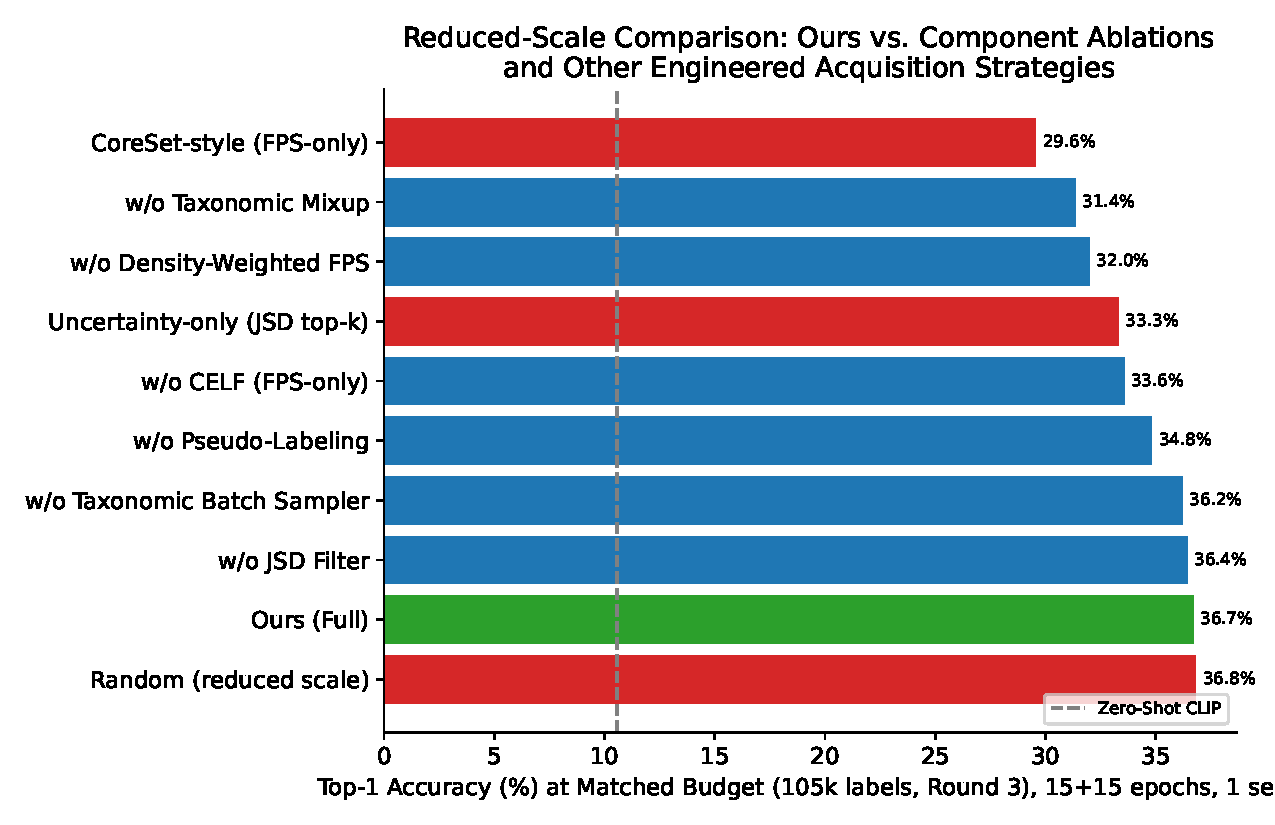
\includegraphics[width=\linewidth]{figs/fig4_engineered_baselines_comparison.pdf}
\caption{Reduced-scale comparison. Ours clearly beats other engineered heuristics (CoreSet-style, uncertainty-only) and every component ablation; reduced-scale random sampling remains a near-tie, consistent with the matched-epoch result in Fig.~\ref{fig:matched} once training budget is properly controlled.}
\label{fig:engineered}
\end{figure}

Two patterns are worth separating clearly. First, \textbf{ours\_full beats every other engineered heuristic by a wide margin}: $+3.38$ points over uncertainty-only sampling, $+7.14$ points over CoreSet-style diversity alone, and a clear margin over every component ablation except the two weakest (JSD filter, $-0.27$; taxonomic sampler alone, $-0.48$, both plausibly within single-seed noise). Second, \textbf{random sampling is the one strategy our pipeline does not clearly beat}, here or in the fully-controlled comparison of Section~\ref{sec:matched}. The four components with the largest individual ablation margins — Taxonomic Mixup ($-5.35$), Density-Weighted FPS ($-4.70$), CELF ($-3.14$), and Pseudo-Labeling ($-1.88$) — are the same components that let the full pipeline outperform \emph{other smart heuristics}; they do not, on this evidence, resolve the gap against random sampling.

\subsection{A Note on the Single-Shot Supervised Control}
A single-shot control — 175k labels selected randomly in one round with no active learning loop, evaluated after one round of the standard 40+40 epoch schedule — reaches $45.68\% \pm 0.10\%$ Top-1 (3 seeds), below both \textbf{ours\_full} and matched-epoch random sampling. We do not read this as evidence that the iterative round structure itself is responsible for the gap: this control receives only one round's worth of total training (40+40 epochs once) against five rounds' worth for the other two arms (each round retrains fresh), so the comparison confounds ``no active learning loop'' with ``five times less total training.'' We report the number for completeness but do not draw a causal conclusion from it.

\subsection{Memory-Wall Measurement}
\label{sec:memwall}
Independent of the acquisition-strategy question, we instrument the acquisition step directly with \texttt{torch.cuda.max\_memory\_allocated()} and compare it, per round, against an analytical estimate of the memory a naive dense $O(N^2)$ pairwise similarity computation would require over the same candidate pool. Fig.~\ref{fig:memwall} shows the result, averaged over 3 seeds of \textbf{ours\_full}. In round 1, before JSD-based pre-filtering reduces the pool, the naive estimate is $596.0$~GB against a measured actual peak of $6.24$~GB — a $96\times$ reduction. In rounds 2 through 5, with the pool already reduced to at most $3\times$ the round budget, the naive estimate drops to roughly $41$~GB against a measured $\sim 3.02$~GB, a consistent $14\times$ reduction. This measurement holds regardless of how the acquisition-strategy comparison resolves: CELF's batching is what makes exact submodular maximization tractable at this scale at all, independent of whether that maximization ultimately beats random sampling.

\begin{figure}[t]
\centering
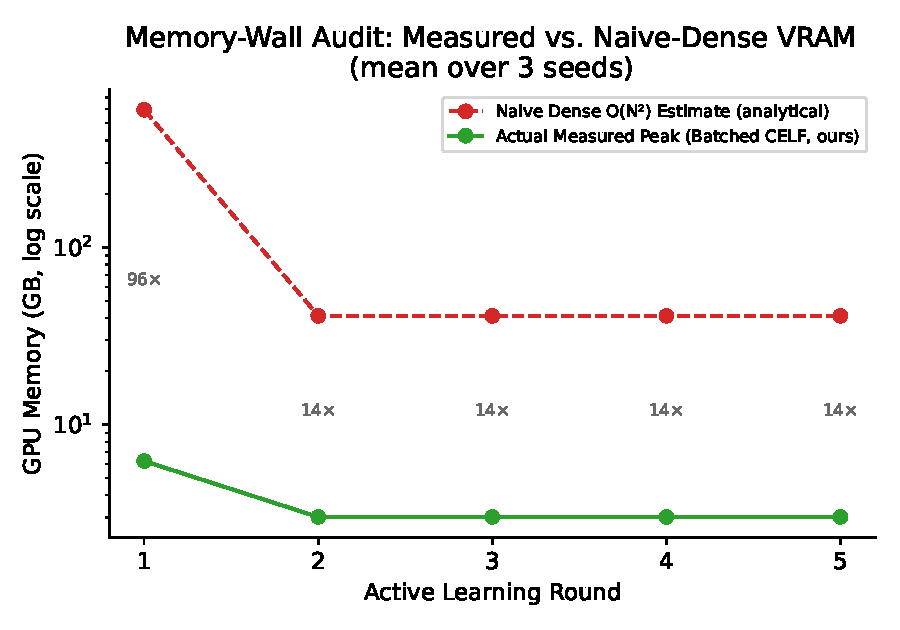
\includegraphics[width=\linewidth]{figs/fig5_memory_wall.pdf}
\caption{Measured peak GPU memory during acquisition vs.\ the analytical naive-dense $O(N^2)$ estimate, log scale, mean over 3 seeds.}
\label{fig:memwall}
\end{figure}

\subsection{Pseudo-Label Leakage and Accuracy Audit}
\label{sec:pseudoaudit}
We snapshot ground-truth labels for the entire training pool \emph{before} any pseudo-label can overwrite them, and assert programmatically, at runtime, that the train and test splits never overlap. Every pseudo-label harvested is compared against this frozen ground truth as a diagnostic only, never fed back into selection or training. Fig.~\ref{fig:pseudoaudit} shows this-round pseudo-label accuracy rising from $89.3\%$ (round 2) to $96.2\%$ (round 5), with cumulative accuracy over all currently-held pseudo-labels remaining above $89\%$ throughout and reaching $94.2\%$ by round 5 — indicating the $\geq 90\%$ confidence threshold is a reasonably well-calibrated proxy for correctness at this scale, and that the loop is not silently degrading label quality as pseudo-labels accumulate. Like the memory-wall measurement, this result is independent of how the acquisition-strategy question resolves, since pseudo-labeling operates identically regardless of which images entered the labeled set.

\begin{figure}[t]
\centering
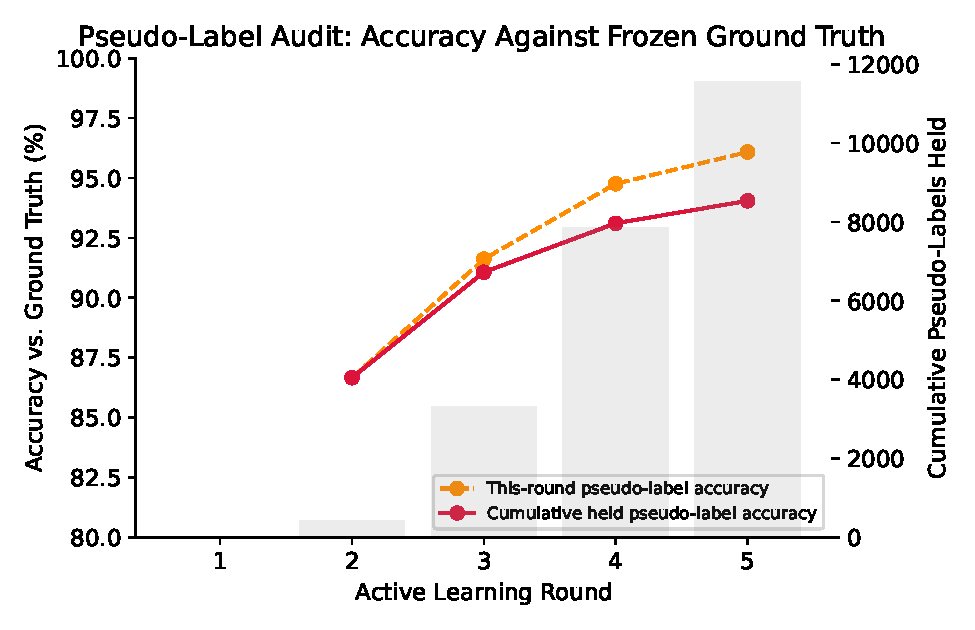
\includegraphics[width=\linewidth]{figs/fig6_pseudo_label_audit.pdf}
\caption{Pseudo-label accuracy against frozen ground truth, and cumulative volume harvested.}
\label{fig:pseudoaudit}
\end{figure}

\section{Discussion and Limitations}
\label{sec:limitation}

\textbf{We have not yet isolated which specific stage of the acquisition pipeline drives the gap against random sampling.} Section~\ref{sec:matched} proposes the JSD pre-filter's hardness-skew, compounded by cold-start unreliability, as the leading hypothesis, but the reduced-scale ablation removing the JSD filter alone (Table~\ref{tab:ablation}) shows only a small effect, which is not fully consistent with the JSD filter alone being responsible. A matched-epoch ablation isolating each of the JSD filter, density-weighted FPS, and CELF individually against matched-epoch random sampling — rather than only against each other at reduced scale — is the direct follow-up experiment this result calls for, and the natural next use of the dispatcher infrastructure described in Section~\ref{sec:dispatch}.

\textbf{The reduced-scale ablation and baseline comparisons (Section~\ref{sec:ablation}) remain single-seed.} Only the two headline arms — \textbf{ours\_full} and the matched-epoch random-sampling control — have 3-seed confirmation. The seven component ablations, the uncertainty-only baseline, and the CoreSet-style baseline are each a single run at reduced schedule (3 rounds, 15+15 epochs), chosen to keep total compute tractable while still isolating each component's individual contribution. The largest ablation margins (Taxonomic Mixup, Density-Weighted FPS, CELF) are unlikely to be pure noise given their size relative to the near-zero margins on the two weakest ablations (JSD filter, taxonomic sampler alone) run under identical conditions, but we would treat exact magnitudes here with more caution than the fully-powered comparison in Section~\ref{sec:matched}.

\textbf{A full BADGE~\cite{ash2020badge} comparison remains future work,} alongside a matched-epoch, multi-seed rerun of the component ablations once compute allows — the acquisition dispatcher (Section~\ref{sec:dispatch}) makes both a configuration change rather than new engineering.

\section{Conclusion}
We built a multi-modal active learning pipeline for extreme fine-grained classification and asked, under a fully-controlled, 3-seed-per-arm comparison, whether its acquisition strategy actually beats random sampling. The honest answer is no: random sampling leads at every one of five active learning rounds once epochs, rounds, label budget, and seed count are matched, by $1.8$ to $4.9$ points Top-1 accuracy, with tighter variance than our own method at every round. The same pipeline clearly beats other engineered acquisition heuristics under identical reduced-scale conditions — uncertainty-only sampling by $3.4$ points, CoreSet-style diversity alone by $7.1$ points — indicating the components are not broken, but rather that sophistication among heuristics does not translate into an advantage over no heuristic at all in this setting. This finding is consistent with, and extends, a small but important line of work showing that many published active learning methods fail to beat random sampling once fairly compared~\cite{mittal2019parting,munjal2022towards}.

Independent of that result, a measured Memory-Wall audit confirms a $14$--$96\times$ real VRAM reduction from batched submodular acquisition against a dense $O(N^2)$ baseline, and a leakage-audited pseudo-labeling loop holds $89$--$96\%$ accuracy against frozen ground truth throughout training. We release the acquisition-strategy dispatcher and audit infrastructure underlying every comparison in this paper so that running a matched-budget random-sampling control is a configuration change, not a second engineering project — infrastructure we believe the active learning literature would benefit from adopting more broadly.

\begin{thebibliography}{00}
\bibitem{vanhorn2018inaturalist} G. Van Horn, O. Mac Aodha, Y. Song, Y. Cui, C. Sun, A. Shepard, H. Adam, P. Perona, and S. Belongie, ``The iNaturalist species classification and detection dataset,'' in \emph{Proc. IEEE Conf. Computer Vision and Pattern Recognition (CVPR)}, 2018, pp. 8769--8778.

\bibitem{nemhauser1978analysis} G. L. Nemhauser, L. A. Wolsey, and M. L. Fisher, ``An analysis of approximations for maximizing submodular set functions---I,'' \emph{Mathematical Programming}, vol. 14, no. 1, pp. 265--294, 1978.

\bibitem{leskovec2007cost} J. Leskovec, A. Krause, C. Guestrin, C. Faloutsos, J. VanBriesen, and N. Glance, ``Cost-effective outbreak detection in networks,'' in \emph{Proc. 13th ACM SIGKDD Int. Conf. Knowledge Discovery and Data Mining}, 2007, pp. 420--429.

\bibitem{khosla2020supcon} P. Khosla, P. Teterwak, C. Wang, A. Sarna, Y. Tian, P. Isola, A. Maschinot, C. Liu, and D. Krishnan, ``Supervised contrastive learning,'' \emph{Advances in Neural Information Processing Systems (NeurIPS)}, vol. 33, pp. 18661--18673, 2020.

\bibitem{bae2021selfcon} S. Bae, S. Kim, J. Ko, G. Lee, S. Noh, and S. Y. Yun, ``Self-contrastive learning: Single-viewed supervised contrastive framework using sub-network,'' \emph{arXiv preprint arXiv:2106.15499}, 2021.

\bibitem{he2020momentum} K. He, H. Fan, Y. Wu, S. Xie, and R. Girshick, ``Momentum contrast for unsupervised visual representation learning,'' in \emph{Proc. IEEE/CVF Conf. Computer Vision and Pattern Recognition (CVPR)}, 2020, pp. 9729--9738.

\bibitem{sener2018coreset} O. Sener and S. Savarese, ``Active learning for convolutional neural networks: A core-set approach,'' in \emph{International Conference on Learning Representations (ICLR)}, 2018.

\bibitem{ash2020badge} J. T. Ash, C. Zhang, A. Krishnamurthy, J. Langford, and A. Agarwal, ``Deep batch active learning by diverse, uncertain gradient lower bounds,'' in \emph{International Conference on Learning Representations (ICLR)}, 2020.

\bibitem{sohn2020fixmatch} K. Sohn, D. Berthelot, N. Carlini, Z. Zhang, H. Zhang, C. Raffel, E. D. Cubuk, A. Kurakin, and C.-L. Li, ``FixMatch: Simplifying semi-supervised learning with consistency and confidence,'' \emph{Advances in Neural Information Processing Systems (NeurIPS)}, vol. 33, pp. 596--608, 2020.

\bibitem{mittal2019parting} S. Mittal, M. Tatarchenko, \"O. \c{C}i\c{c}ek, and T. Brox, ``Parting with illusions about deep active learning,'' \emph{arXiv preprint arXiv:1912.05361}, 2019.

\bibitem{munjal2022towards} P. Munjal, N. Hayat, M. Hayat, J. Sourati, and S. Khan, ``Towards robust and reproducible active learning using neural networks,'' in \emph{Proc. IEEE/CVF Conf. Computer Vision and Pattern Recognition (CVPR)}, 2022, pp. 223--232.

\end{thebibliography}

\end{document}
